
\section{Calibração Intrínseca}

\begin{figure}[H]
	\centering
	\begin{subfigure}[H]{0.49\textwidth}
		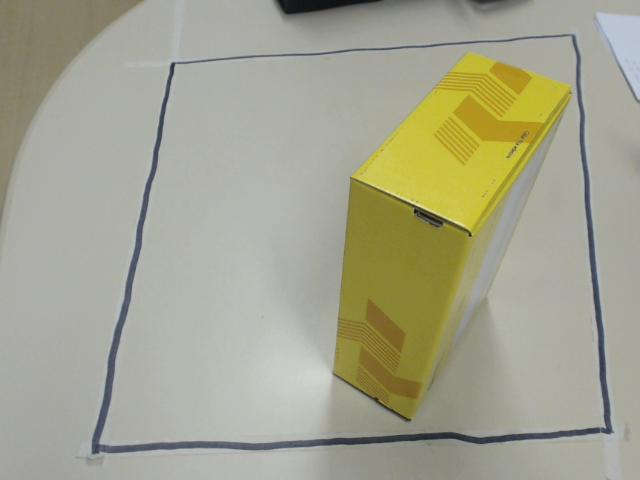
\includegraphics[width = \textwidth]{../../data/i7_L.jpg}
		\caption{Vista esquerda.}
		\label{fig:i7_L}
	\end{subfigure}
	\begin{subfigure}[H]{0.49\textwidth}
		\centering
		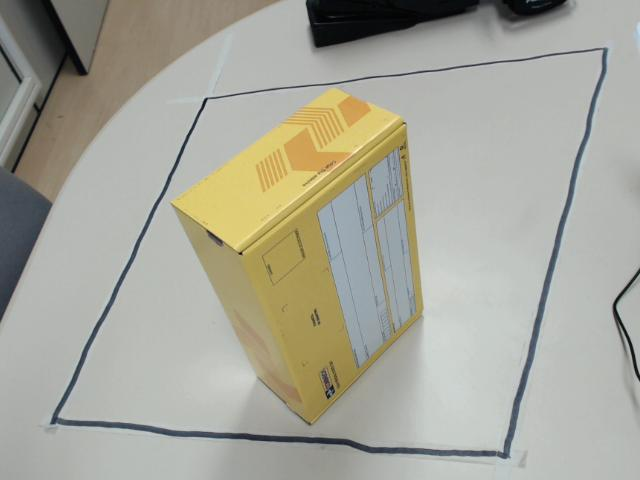
\includegraphics[width = \textwidth]{../../data/i7_R.jpg}
		\caption{Vista direita.}
		\label{fig:i7_R}
	\end{subfigure}
\end{figure}

\subsection{Obtenção de pontos}

\begin{figure}[H]
	\centering
	\begin{subfigure}[H]{0.49\textwidth}
		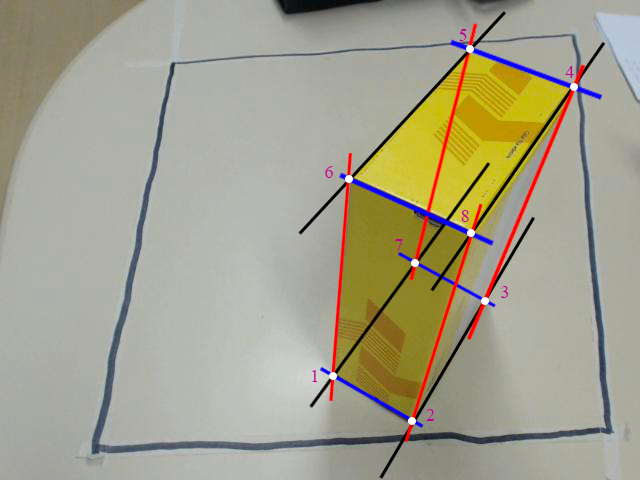
\includegraphics[width = \textwidth]{../../data/i7_L_axis.png}
		\caption{Vista esquerda.}
		\label{fig:i7_L_axis}
	\end{subfigure}
	\begin{subfigure}[H]{0.49\textwidth}
		\centering
		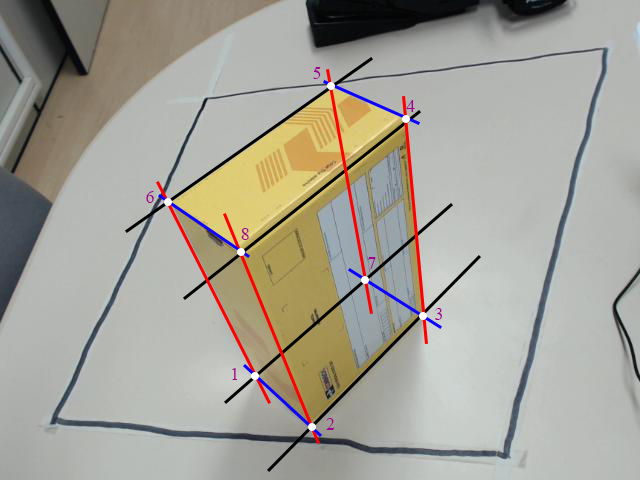
\includegraphics[width = \textwidth]{../../data/i7_R_axis.png}
		\caption{Vista direita.}
		\label{fig:i7_R_axis}
	\end{subfigure}
\end{figure}


\section{Transformação entre às câmeras}

A matriz de rotação e o vetor de translação entre a câmera e o sistema de coordenadas do mundo podem ser representadas na forma de transformações homogêneas, que compactam a informação de rotação e translação, sendo construída com base em \eqref{eq:th}.

\begin{equation}
	\+T = \begin{bmatrix}
	&	\+R_{[3\times 3]} & & \vec{t}_{[3\times 1]} \\
		0 & 0 & 0 & 1
	\end{bmatrix}_{[4\times 4]}
	\label{eq:th}
\end{equation}

Para a transformação entre os \textit{frames} $\{2\}$ e $\{1\}$, tem-se \eqref{eq:th21}.

\begin{equation}
\+T_{2/1} = \begin{bmatrix}
	& \+R_{2/1} & & \vec{t}_{2/1} \\
	0 & 0 & 0 & 1
\end{bmatrix}
\label{eq:th21}
\end{equation}

De acordo com a propriedade algébrica das transformações homogêneas, a transformação do \textit{frame} $\{0\}$ para o $\{2\}$ pode ser decomposta no produto da transformação do \textit{frame} $\{0\}$ para o $\{1\}$, e do   \textit{frame} $\{1\}$ para o $\{2\}$.

\begin{equation}
	\+T_{0/2} = \+T_{2/1} \+T_{1/0} \therefore \+T_{2/1} = \+T_{0/2} \+T_{1/0} = \+T_{0/2} \+T^{-1}_{0/1}
\end{equation}

Dessa forma, uma vez que se conhece a transformação da câmera na vista esquerda para o sistema do mundo, e a transformação da câmera na vista direita para o sistema do mundo, a tranformação entre as duas câmeras pode ser encontrada da forma \eqref{eq:tfLR}.

\begin{equation}
	\+T_{R/L} = \+T_{R/0}\+T_{0/L} =  \+T_{R/0}\+T_{L/0}^{-1}
	\label{eq:tfLR}
\end{equation}




